\chapter{Implementierung}
\label{chapter_Implementierung}

\section{Hardware}

\section{Software}

Die Installation der Linux Software erfolgt mittels des Terminalemulator PuTTY \cite{putty}. Mit \mbox{PuTTY} wird eine \ac{SSH} Verbindung zu dem BeagleBone Black aufgebaut, wodurch ein direkter Zugriff auf das Linux Terminal des BeagleBone Black möglich ist. Mit dem Linux Paketmanager kann bei aktiver Internetverbindung die benötigte Software installiert werden.\ 

Bei der Implementierung der eigenen Software wird wie in Kapitel \ref{chapter_Design} erwähnt, die Qt C++ Klassenbibliothek in der Version 4.8.6 verwendet. Für die komfortable Programmierung eignet sich der Qt Creator als Entwicklungsumgebung sehr gut. Er bietet die Möglichkeit direkt in der Entwicklungsumgebung eine Toolchain einzurichten. Diese erlaubt eine Programmierung des Codes auf einem normalen Windows Rechner, wobei der Code anschließend automatisch übersetzt und auf dem Zielsystem über eine \ac{SSH} Verbindung installiert wird. Verwendet wird dabei ein frei verfügbarer \ac{GCC}.\\
Das Steuerungssoftware teilt sich in einen sequentiellen Prozess für die Abfrage und Speicherung der Messwerte, sowie einen Event gesteuerten Prozess für die \ac{GUI} und die externe Kommunikation für die Fernzugriffe. 
Die beiden Programmteile können unabhängig von einander agieren und kommunizieren ausschließlich über Signale und Slots (siehe Abschnitt \ref{QtSignaleSlots}). Durch diese Kapselung ist es möglich die beiden Programmteile durch andere Lösungen auszutauschen, welche lediglich die selben Signale und Slots unterstützen müssen.

\subsection{Systemkonfiguration}

Beim Hochfahren des Mess-Servers sorgt das Linux Hintergrundprogramm systemd für die Ausführung alle nötigen Prozesse. Um zusätzlich die Steuerungssoftware zu starten, wird ein neuer Service erstellt und dem systemd mitgeteilt.\\

\begin{lstlisting}[caption={Systemd Service},label=lst_SystemdService]
[Unit]
Description=Boot Setup
[Service]
TimeoutStartSec=300
EnvironmentFile=/etc/Bootsetup.conf
ExecStart=/usr/bin/Bootsetup
Restart=always
RestartSec=30
[Install]
WantedBy=multi-user.target
\end{lstlisting}

Im Quellcode \ref{lst_SystemdService} ist die Konfiguration des Services zu sehen. Er wird beim Systemstart automatisch gestartet und führt anschließend ein Script aus, dass das System konfiguriert und die Qt Anwendung startet. Des Weiteren wird der Service automatisch erneut ausgeführt, falls ein Fehler, der die Qt Anwendung beendet, auftritt. Dadurch soll sichergestellt werden, dass das System jederzeit verfügbar ist.\ 

Das Systemstart Script initialisiert zunächst das RS232 Cape, das \ac{RTC} Cape und die Systemuhr. Anschließend führt es die Qt Anwendung aus.\\ 

\begin{lstlisting}[caption={Systemstart Script},label=lst_SystemstartScript]
#!/bin/bash
echo BB-UART4 >/sys/devices/bone_capemgr.*/slots
echo BBB-RTC-01:00A1 >/sys/devices/bone_capemgr.*/slots
sleep 60
hwclock -s -f /dev/rtc1
sleep 60
cd /root/Progs
./LTT_MeasMaster_GUI -qws
\end{lstlisting}

Im Quellcode \ref{lst_SystemstartScript} ist das Systemstart Script zu sehen. Für die Initialisierung des RTC und RS232 Capes erfolgt über den für das BeagleBone Black verfügbaren Cape Manager (capemgr). Der Capemgr \cite{Capemgr} dient zum einfachen Einbinden von Capes in das System. Er lädt unter Anderem die benötigten Treiber und reserviert die nötigen \ac{GPIO} Pins.\ 

Da das BeagleBone Black über keine persistente Uhr verfügt, wird nachdem die beiden Capes initialisiert sind die Systemuhr mithilfe der Uhrzeit des RTC Capes gestellt. Die Uhrzeit muss zu jeder Zeit korrekt sein, damit das System fehlerfrei funktioniert.\\
Nach der Konfiguration wird die Qt Steuerungssoftware ausgeführt. Sie wird dabei weiterhin vom systemd überwacht und im Fehlerfall neu gestartet.\ 

Alle Log-Nachrichten werden dabei in die Logdatei des systemd geschrieben. Die dadurch anfallenden Datenmengen überschreiten dabei schnell die Kapazitäten der Hardware des BeagleBone Blacks. Deshalb wird zur Organisation der Logdateien die im Linux Betriebssystem mitgelieferte Software logrotate \cite{logrotate} eingesetzt. Logrotate übernimmt die automatische Rotation, Kompression und Löschung von Logdateien.\\

\begin{lstlisting}[caption={Logrotate},label=lst_Logrotate]
/var/log/daemon.log
{
        size 100M
        weekly
        rotate 4
        compress
}
\end{lstlisting}

Im Quellcode \ref{lst_Logrotate} ist die entsprechende Konfiguration zu sehen. Die maximale Größe der Logdateien ist dabei auf 100MB beschränkt um den internen Speicher von 4GB nicht zu sehr zu belasten. Wird diese Größe überschritten wird die Logdatei rotiert. Dabei wird ein Backup der aktuellen Logdatei erstellt und eine neue angelegt. Des Weiteren wird die Logdatei einmal pro Woche unabhängig von der Größe rotiert. Bei der Rotation werden die letzten 4 Logdateien gespeichert. Kommt eine Weitere dazu, wird die älteste gelöscht. Die maximale Größe von 100MB stellt dabei nur selten das Limit dar. So stehen die Logdateien für etwa 4 Wochen rückblickend zur Verfügung.



\subsection{RS232 Kommunikation}

Die Kommunikation von dem Mess-Server mit den Mess-Clients erfolgt sequentiell. Der Mess-Server stellt eine Anfrage und wartet anschließend für eine festgelegte Zeit auf eine Antwort. Die Antwort enthält bei fehlerfreier Kommunikation das invertierte Read/Write-Bit, sowie die gleiche RS232 Adresse und den selben Befehl/Unterbefehl wie bei der Anfrage. Bei einer Leseanfrage enthält die Antwort zusätzlich noch die angeforderten Daten.\\

\begin{figure}[H]
\begin{center}
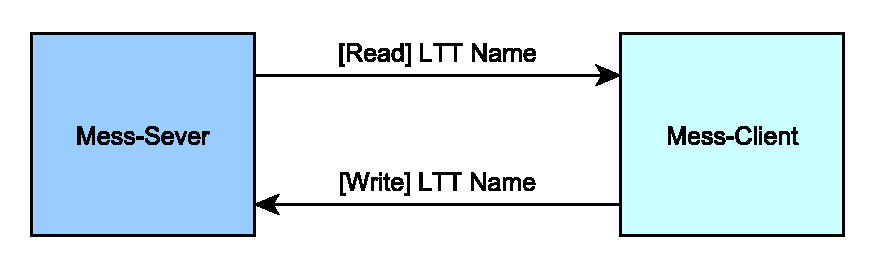
\includegraphics[width=0.7\textwidth ]{img/general/RS232Uebertragung.pdf}
\caption{RS232 Kommunikation: Leseanfrage}
\label{figure_RS232Kommunikation}
\end{center}
\end{figure}

Um Fehler bei der Kommunikation zu vermindern und die Erfolgschancen zu erhöhen, müssen fehlerhafte Übertragungen erkannt und wenn möglich korrigiert werden. Die Erkennung von Fehlern geschieht durch die Auswertung der Antwort eines Mess-Clients.

Dabei können drei Szenarien auftreten:
\begin{itemize}
\item Keine Antwort: Innerhalb des Zeitlimits wurde keine Antwort empfangen.
\item Falsche Antwort: Innerhalb des Zeitlimits wurde eine Antwort empfangen, jedoch entspricht sie nicht den Erwartungen.
\item Prüfsummen-Fehler: Innerhalb des Zeitlimits wurde eine Antwort empfangen, jedoch ist die Prüfsumme nicht korrekt.
\end{itemize}

Zur Korrektur dieser Fehler werden Anfragen bis zu fünfmal in einem festgelegtem zeitlichen Abstand wiederholt gesendet. Sollte die Übertragung weiterhin fehlerhaft sein, ist der Mess-Client entweder nicht erreichbar oder es gibt einen Adresskonflikt auf dem RS232 Bus. Bei einem Adresskonflikt haben mehrere zwei oder mehr Mess-Clients die selbe RS232 Adresse. Das führt dazu, dass beide Mess-Clients auf die selben Anfragen reagieren und ihre Antworten sich auf dem RS232 Bus überlagern.




\subsection{Datenbank}

Die Datenbank muss aus dem Netzwerk erreichbar sein, damit die Messdaten von einem PC-Client abgerufen werden können. Bei einem MySQL Server ist dies jedoch nicht von Grund auf gegeben. Standardmäßig akzeptiert der MySQL Server nur Anfragen über die Localhost Adresse (IP-Adresse: 127.0.0.1). Deshalb müssen die Zugriffsrechte erst erteilt werden.\\

\begin{lstlisting}[caption={MySQL Zugriffsrechte},label=lst_MySQLZugriffsrechte]
GRANT ALL ON *.* to root@'%' IDENTIFIED BY 'toor';
\end{lstlisting}

Mit dem Befehl im Quellcode \ref{lst_MySQLZugriffsrechte} erhalten alle Nutzer die sich mit dem Benutzernamen \textit{root} und dem Passwort \textit{toor} identifizieren, vollen Zugriff auf alle Datenbanken. Somit ist es möglich von überall aus eine Verbindung zum Datenbankserver aufzubauen und sämtlichen Daten abzurufen.\\

Über einen langen Betriebszeitraum können sich große Mengen an Daten in der Datenbank ansammeln. Das hat zur Folge, dass die SQL-Abfragen nach nach bestimmten Daten sehr lange dauern können. Um dem Vorzubeugen werden Indexe für häufig abgefragte Daten erstellt.\\

\begin{lstlisting}[caption={MySQL Index},label=lst_MySQLIndex]

CREATE INDEX measurement_time_idx on Measurement(Time);

\end{lstlisting}


Der Quellcode \ref{lst_MySQLIndex} zeigt die Erzeugung eines Indexes. Der Index mit dem Namen \textit{measurement\_time\_idx} wird für die Spalte \textit{Time} in der Tabelle \textit{Measurement} angelegt. Vor Allem in der Tabelle \textit{Measurement} können sehr schnell große Mengen an Daten anfallen.\\
Der Index für die Spalte \textit{Time} ist besonders gut geeignet. Denn um herauszufinden wann die letzte Messungen durchgeführt wurde, muss aus der Tabelle \textit{Measurement} das Messergebnis mit dem aktuellsten Zeitstempel ermittelt werden. Diese Abfrage kann bei 2 Millionen Einträgen ohne Index bis zu  2 Minuten dauern. Mit dem Index kann sie auf 4 Sekunden reduziert werden.

Wenn ein Board gelöscht wird, werden alle dazugehörigen Datenbankeinträge aus den anderen Tabellen gelöscht. Das soll unnötigen Daten in der Datenbank vorbeugen. Dafür sind die Fremdschlüssel in allen Tabellen außerhalb der D\_Board Tabelle mit dem Constraint \textit{ON DELETE CASCADE} versehen. Die sorgt für eine Löschung des betroffenen Eintrages, falls das referenzierte Attribut gelöscht wird. Da die Tabellen Setting und Pattern keine eigenen Verweise zu der Tabelle D\_Board haben, ist für diese Kaskadierung ein Trigger notwendig. \\
Ein Trigger ist ein an eine Reaktion auf ein Ereignis. Das Ereignis ist die Löschung eines Eintrags in der D\_Board Tabelle. Daraufhin sollen die dazugehörigen Einträge in der Setting und der Pattern Tabelle gelöscht werden. Dafür wird ein Trigger erstellt (siehe Quellcode \ref{lst_Trigger}).\\

\begin{lstlisting}[caption={onBoardDelete Trigger},label=lst_Trigger]
Create Trigger onBoardDelete before delete on D_Board 
for each row 
Begin 
delete from Setting 
	where p_id = old.f_Settingid;
delete from Pattern 
	where p_id = old.f_Patternid;
end;
\end{lstlisting}








backup und restore ?

QT crosscompile?



LCD display energiesparmodus, wecken durch geste


hw clock aktualisierung bei ntp verbindung



Captive Portal dnsmasq ,lighttpd



\subsection{Webinterface}

Das Webinterface soll nach der Verbindung über den WLAN Hotspot ohne eine spezielle Adresse manuell im Webbrowser aufrufen zu müssen erreichbar sein. Dafür wird der DNS Server dnsmasq so konfiguriert, dass alle Anfragen auf den Webserver umgeleitet werden.

\begin{lstlisting}[caption={MySQL Index},label=lst_MySQLIndex]

interface=wlan0
dhcp-range=wlan0,192.168.10.10,192.168.10.50,4h
address=/#/192.168.10.1

\end{lstlisting}


\subsection{Anwendung zur Messdatenauswertung}

\begin{figure}[H]
\begin{center}
\includegraphics[width=0.7\textwidth ]{img/general/PCClientMain.PNG}
\caption{RS232 Kommunikation: Leseanfrage}
\label{figure_RS232Kommunikation}
\end{center}
\end{figure}


\begin{figure}[H]
\begin{center}
\includegraphics[width=0.7\textwidth ]{img/general/PCClientBoard.PNG}
\caption{RS232 Kommunikation: Leseanfrage}
\label{figure_RS232Kommunikation}
\end{center}
\end{figure}
